%\documentclass[12pt]{amsart}
\documentclass[12pt]{report}


%\usepackage[margin=0.8in]{geometry} % see geometry.pdf on how to lay out the page. There's lots.
\usepackage{geometry} % see geometry.pdf on how to lay out the page. There's lots.
\usepackage{graphicx}
\usepackage{subcaption} %These packages gives the author the ability to have subfigures within figures, or subtables within table floats.
\usepackage{hyperref}
\usepackage{slashed} % Dirac slash notation
\usepackage{amsmath}
\usepackage{authblk}
\usepackage{multirow}

\geometry{a4paper} % or letter or a5paper or ... etc
% \geometry{landscape} % rotated page geometry

% See the ``Article customise'' template for come common customisations

\title{Introduction to Supersymmetry}
\author{Yu-Ting Shen}
\affil{Homer L. Dodge Department of Physics and Astronomy\\
The University of Oklahoma}
\date{} % delete this line to display the current date

%%% BEGIN DOCUMENT
\begin{document}

\maketitle
\tableofcontents


%%%%%
%%%%%
%%%%%
\chapter{Motivations for supersymmetry}
The Standard Model (SM) of particle physics was established since 1970s and it can explain the elementary particles and the interactions that construct our world.
However, the SM is still incomplete and needs to be extended.
In order to extend SM, many different models of new physics are proposed such as technicolor, little Higgs, and supersymmetry.
Among all the possible theories, the supersymmetry (SUSY) \cite{wess_and_zumino} plays an important role.

All the symmetry we know relate bosons to bosons and fermions to fermions but not bosons to fermions.
SUSY is a kind of symmetry that mixes bosons and fermions.
The SUSY theory requires every boson has a fermion partner, and vice versa.
We can extend the SM into its SUSY version which says every SM boson (or fermion) has an fermonic (or bosonic) supersymmetry partner.
In other words, the generators $Q$ of SUSY must turn a bosonic state into a fermonic state, with
\begin{equation}
Q|\mathrm{boson}\rangle = |\mathrm{fermion}\rangle, \qquad 
Q|\mathrm{fermion}\rangle = |\mathrm{boson}\rangle
\end{equation}
which also implies the generators of SUSY are anticommuting operators.

SUSY has the potential to provide explanations for the phenomena which SM cannot explain, for example, hierarch problem, running coupling constants, and candidates of dark matter.
The SM Higgs field has a potential
\begin{equation}
V = m^{2}_{H} |\phi|^{2} + \lambda |\phi|^{2} .
\end{equation}
In order to satisfy electroweak symmetry breaking, the SM requires the vacuum expectation value (VEV) for Higgs field $\phi$ has to be non-zero.
This will occur if $\lambda > 0$ and $m^{2}_{H} < 0$.
It is inferred from experiments that the value of $m^{2}_{H}$ is about $-(100 \textrm{ GeV})^2$, however, the Higgs squared mass parameter $m^{2}_{H}$ also receives large radiative corrections\footnote{$m^{2}_{H} (\textrm{phys}) = m^{2}_{H} (\textrm{bare}) + \delta m^{2}_{H}$, where $\delta m^{2}_{H}$ is the correction.} from particles couple to Higgs field.
Consider a one-loop corrections to $m^{2}_{H}$ due to a fermion in figure \ref{fig: one-loop diagram} and let the Higgs field couples to $f$ with a Lagrangian term $-\lambda_{f} H f \overline{f}$.\footnote{The SM Higgs field $\phi =Re(H - v)/\sqrt{2}$ where $v \simeq 246$ GeV.}
The correction of $m^{2}_{H}$ is given by
\begin{equation}
\delta m^{2}_{H} = - \frac{|\lambda_{f}|^2}{8 \pi^{2}} \Lambda^{2} + \mathcal{O}(m^{2}_{f})
\end{equation}
This term is \textit{quadratically divergent} if $\Lambda$ goes to infinity.
If we replace $\Lambda$ by the Plank scale $M_{P} \sim 10^{19}$ GeV, the correction to $m^{2}_{H}$ is about 30 orders of magnitude larger than the required value of $m^{2}_{H}$.
This is the \textbf{hierarchy problem}, we have to fine tune the vary large loop correction to cancel the very large bare mass.
The SUSY extension of SM says there exists a contribution from the bosonic superpartner, \textit{sfermion}, as shown in figure \ref{fig: sfermion_one-loop_diagram}.
Let the Lagrangian term from the Higgs couples to sfermion, $\widetilde{f}$, is $-\lambda_{\widetilde{f}} |H|^{2} |\widetilde{f}|^{2}$ and gives the correction
\begin{equation}
\delta m^{2}_{H} = \frac{\lambda_{\widetilde{f}}}{16 \pi^{2}} \Lambda^{2} + \mathcal{O}(m^{2}_{\widetilde{f}}) .
\end{equation}
We notice there is a relative minus sign between boson loop and fermion loop contributions to $m^{2}_{H}$.
This provides us a hint that the SUSY extension of SM might solve the hierarchy problem if the bosonic and fermonic contributions can cancel each other.
\begin{figure}[htbp]
\begin{center}
\begin{subfigure}[b]{0.45\textwidth}
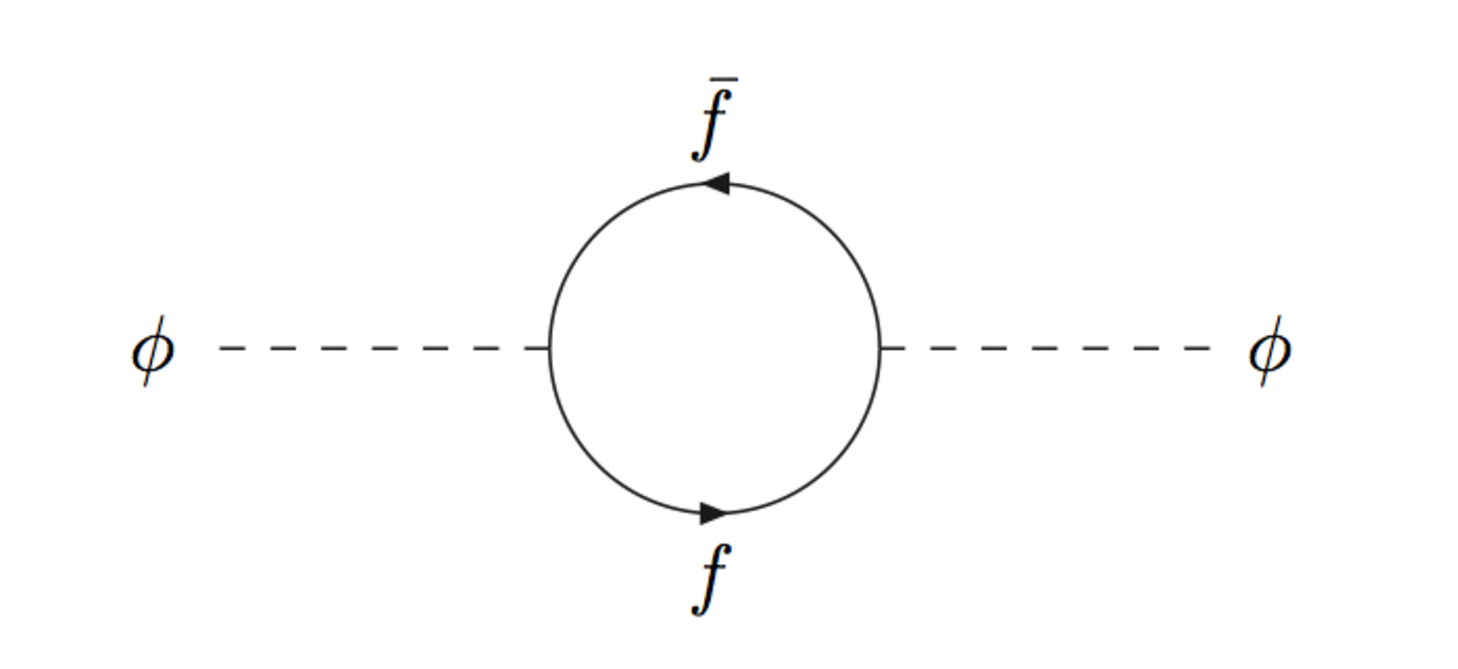
\includegraphics[scale=0.4]{figures/one-loop_diagram.pdf}
\caption{}
\label{fig: one-loop diagram}
\end{subfigure}
~%add desired spacing between images, e. g. ~, \quad, \qquad, \hfill etc.
\begin{subfigure}[b]{0.45\textwidth}
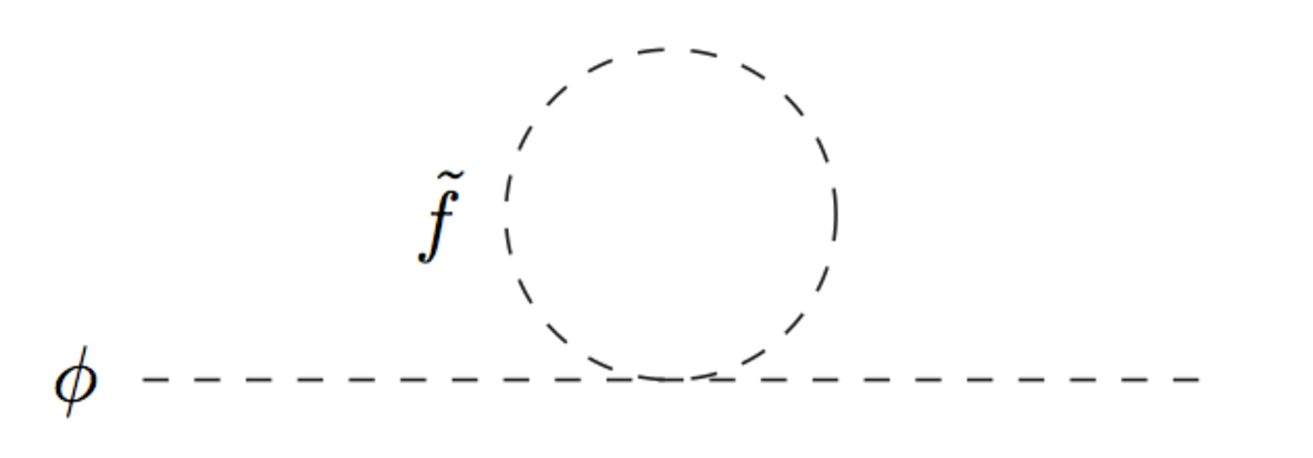
\includegraphics[scale=0.4]{figures/sfermion_one-loop_diagram.pdf}
\caption{}
\label{fig: sfermion_one-loop_diagram} 
\end{subfigure}
\caption{(a) A fermion and anti-fermion contribution to the self-energy of the Higgs boson in the Standard Model. (b) The sfermion loop contribution to the Higgs self-energy. $\widetilde{f}$ stands for sfermion.}
\label{}
\end{center}
\end{figure}

The running coupling constants are functions of energy as shown in the figure \ref{fig: running_coupling_constant}.
The strong coupling $\alpha_{1}$ and the weak coupling $\alpha_{2}$ go down, while the electromagnetic coupling $\alpha_{3}$ goes up.
In Grand Unified Theory (GUT), these three constants should be identical in strength when the energy is above the grand unification scale ($\approx 10^{16}$ GeV).
Although there is no direct evidence shows the coupling constants converge, the theorists still believe it is true.
However, these three constants do not converge in the Minimal Standard Model (MSM). 
If we extend the MSM into its supersymmetric version, Minimal supersymmetric Standard Model (MSSM), they do converge well.
\begin{figure}[htbp]
\begin{center}
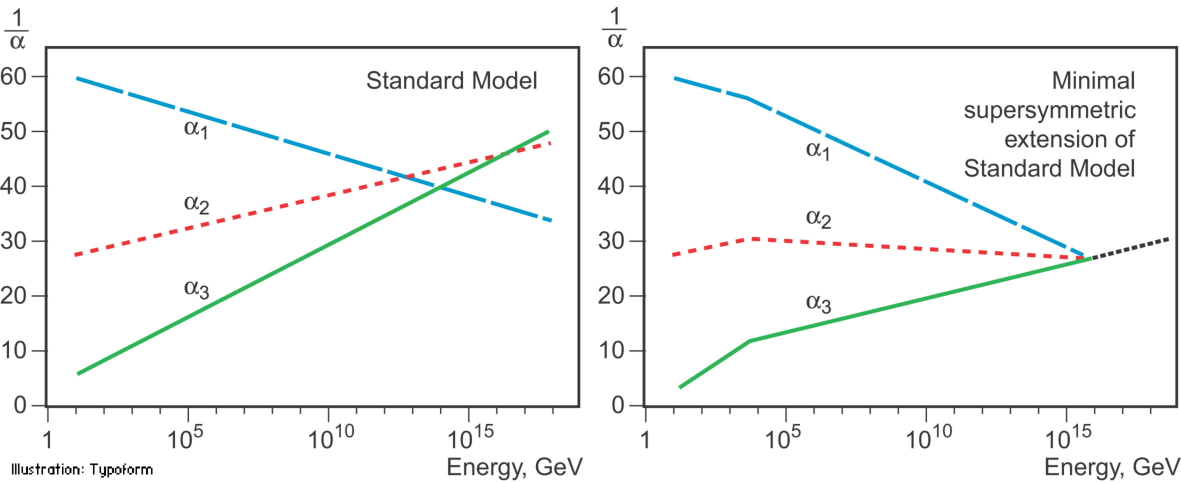
\includegraphics[scale=0.75]{figures/phypub4highen.pdf}
%This figure is from http://www.nobelprize.org/nobel_prizes/physics/laureates/2004/phypub4highen.jpg
\caption{The coupling constants at the GUT scale in the Minimal Standard Model (left) and in Minimal supersymmetric Standard Model (right).
Figure adapted from \url{http://www.nobelprize.org/nobel_prizes/physics/laureates/2004/phypub4highen.jpg}.}
\label{fig: running_coupling_constant}
\end{center}
\end{figure}

Dark matter, which consists $80\%$ of our universe, is a kind of hypothesised matter in cosmology.
Although dark matter cannot be seen directly with telescopes, physicists believe it is a kind of new particles which does not covered in SM.
Many theorists predict the lightest SUSY particles (LSPs) is stable and electrically neutral and they interact with the SM particles weakly.
Because these are also the properties required for dark matter, the SUSY provides potential candidates for dark matter.






%%%%%
%%%%%
%%%%%
\chapter{Superalgebra}
Since supersymmetric theory is based on superalgebra which is an extension of space-time Poincar\'{e} algebra, we first review some basic concepts of Lorentz group, Poincar\'{e} group and spinor notations.
We also describe the other ideas which are frequently used in the calculation of superalgebra.
At the end, we will present representations of the superalgebra, called supermultiplets, both massive and massless. 



\section{Lorentz group}
Since the Lorentz transformation combines rotations and boosts, the infinitesimal Lorentz transformation matrix $U(\vec{\theta}, \vec{\phi}) $ can be written as
\begin{equation}
U(\vec{\theta}, \vec{\phi}) \simeq 1  + i \vec{\theta} \cdot \vec{J} + i \vec{\phi} \cdot \vec{K}
\end{equation}
where $J_{i}$ and $K_{i}$ are rotation and boosts generators, respectively.
The generators of the Lorentz group must satisfy the commutation relations
\begin{equation}
[J_{i}, J_{j}] = i \epsilon_{ijk} J_{k}, \quad
 [K_{i}, K_{j}] = -i \epsilon_{ijk} J_{k}, \quad 
 [J_{i}, K_{j}] = i \epsilon_{ijk} K_{k}
\end{equation}
where $i, j, k = 1, 2, 3$.
It is very convenient to redefine the generators as
\begin{equation}
J^{\pm}_{i} = \frac{1}{2} (J_{i} \pm i K_{i})
\end{equation}
and the commutation relations become
\begin{equation}
[J^{+}_{i}, J^{+}_{j}] = i \epsilon_{ijk} J^{+}_{k}, \quad 
[J^{-}_{i}, J^{-}_{j}] = i \epsilon_{ijk} J^{-}_{k}, \quad 
[J^{+}_{i}, J^{-}_{j}] = 0
\end{equation}
which tell us the Lorentz group can be decomposed into the product of two independent $SU(2)$ groups.



\section{Poincar\'{e} group}
We need the unitary representations of a symmetry group which can preserve the translation probabilities between two eigenstates as measured in different reference frames.
The irreducible representations of the Lorentz group is not unitary, the underlying symmetry group for particle physics is Poincar\'{e} group.
%A space-time transformation includes rotations, boosts and translations in space and time.
%We usually use the energy-momentum operator $P_{\mu}$ to denote the generators of the translation groups.
The Poincar\'{e} group is a product of the Lorentz group and the group of translations in space-time.
We usually use the energy-momentum operator $P_{\mu}$ to denote the generators of the translation groups.
If we define an antisymmetric second rand tensor generator $M_{\mu\nu}$ where the six components are the six Lorentz group generators, with $M_{ij} = \epsilon_{ijk} J_{k}$ and $M_{0i} = - M_{i0} = -K_{i}$.
Then the commutation relations of Poincar\'{e} groups are
\begin{align}
[P_{\mu}, P_{\nu}] &= 0 ,\\
[M_{\mu \nu}, P_{\lambda}] &= i (g_{\nu \lambda} P_{\mu} - g_{\mu \lambda} P_{\nu}) ,\\
[M_{\mu \nu}, M_{\rho \sigma}] &= -i (g_{\mu \rho} M_{\nu \sigma} - g_{\mu \sigma} M_{\nu \rho} - g_{\nu \rho} M_{\mu \sigma} + g_{\nu \sigma} M_{\mu \rho}) .
\end{align}



\section{Spinors: Dirac, Magorana and Weyl fermion fields}
The general state of a spin-1/2 particle can be expressed as a two-component column matrix, called \textbf{spinor}:
\begin{equation}
\chi = c_{+} \chi_{+} + c_{-} \chi_{-} = \left(\begin{array}{c}c_{+} \\c_{-}\end{array}\right)
\end{equation}
with
\begin{equation}
\chi_{+} = \left(\begin{array}{c}1 \\0\end{array}\right), \quad 
\chi_{-} = \left(\begin{array}{c}0 \\1\end{array}\right)
\end{equation}
representing spin up and spin down, respectively.

A \textbf{bi-spinor} is an object that consists of two spinors which belong to two different SU(2) groups.
If a four-component field $\psi_{D}$ is a solution of the Dirac equation $(i \gamma^{\mu} \partial_{\mu} - m) \psi  = 0$, we call $\psi_{D}$ is a \textbf{Dirac spinor} which transforms under boosts and rotations according to:
\begin{equation}
S^{0i} = \frac{i}{4} [\gamma^{0}, \gamma^{i}] , \quad 
S^{ij} = \frac{i}{4} [\gamma^{i}, \gamma^{j}] \equiv \frac{1}{2} \epsilon^{ijk} \Sigma^{k} .
\end{equation}
In stead of using a four-component column matrix, we can express $\psi_{D}$ in terms of bi-spinors:
\begin{equation}
\psi_{D} = \left(\begin{array}{c} \psi_{1} \\ \psi_{2} \\ \psi_{3} \\ \psi_{4} \end{array}\right) = \left(\begin{array}{c} \psi_{L} \\ \psi_{R} \end{array}\right)
\end{equation}
where
\begin{equation}
\psi_{L} = \left(\begin{array}{c} \psi_{1} \\ \psi_{2} \end{array}\right), \quad 
\psi_{R} = \left(\begin{array}{c} \psi_{3} \\ \psi_{4} \end{array}\right)
\end{equation}
are the left-handed and right-handed \textbf{Weyl spinors}.
They transform under infinitesimal rotations $\vec{\theta}$ and boots $\vec{\beta}$ are
\begin{eqnarray}
\psi_{L} \to \psi_{L}' = (1 - i \vec{\theta} \cdot \frac{\vec{\sigma}}{2} - \vec{\beta} \cdot \frac{\vec{\sigma}}{2}) \psi_{L} ;\\
\psi_{R} \to \psi_{R}' = (1 - i \vec{\theta} \cdot \frac{\vec{\sigma}}{2} + \vec{\beta} \cdot \frac{\vec{\sigma}}{2}) \psi_{R} .
\end{eqnarray}
It is very convenient to choice Weyl representation such that Weyl fermion fields (i.e. Weyl spinors) can be seen as the building blocks for any fermion filed.

Majorana found that If we choose all non-zero elements in all $\gamma$ matrices are purely imaginary, we can obtain a \textit{real} solution $\widetilde{\psi}_{M}$ for Dirac equation \cite{majorana}.
A Majorana fermion field is defined through the Majorana condition
\begin{equation}
\widetilde{\psi}_{M} = \widetilde{\psi}^{*}_{M} .
\end{equation}
in Majorana representation.\footnote{We use tilde notation on the top to present Majorana representation.}
We can use similarity transformation to rewrite Majorana condition in a general representation as
\begin{equation}
%\psi = \gamma_{0} C \psi^{*}
\psi = C \overline{\psi}^{T}
\end{equation}
which is saying a Majorana spinor is its own charge conjugate.
We can express a Majorana fermion field in terms of left-handed and right-handed Weyl spinors
\begin{equation}
\psi_{M} = \left( \begin{array}{c} \xi_{\alpha}\\ \overline{\xi}^{\dot{\alpha}} \end{array} \right) = \left( \begin{array}{c} \xi_{\alpha}\\0\end{array} \right) + \left( \begin{array}{c}0\\ \overline{\xi}^{\dot{\alpha}} \end{array} \right) = \psi_{W, L} + \psi_{W, R}
\end{equation}
%where the right-handed Weyl spinor $\xi_{\alpha}$ is the Lorentz-covariant conjugate of the left-handed Weyl spinor.
where the right-handed Weyl spinor $\overline{\xi}^{\dot{\alpha}}$ is the Hermitian conjugate of the left-handed Weyl spinor $\xi_{\alpha}$.

Because the spinors anti-commute, we can derive the following identities for two spinors $\psi$ and $\chi$:
\begin{align}
& \psi \chi = \chi \psi, \quad 
\overline{\psi} \overline{\chi} = \overline{\chi} \overline{\psi}, \quad 
(\psi \chi)^{\dagger} = \overline{\psi} \overline{\chi} \notag \\
& \chi \sigma^{\mu} \overline{\psi} = - \overline{\psi} \overline{\sigma}^{\mu} \chi, \quad 
(\chi \sigma^{\mu} \overline{\psi})^{\dagger} = \psi \sigma^{\mu} \overline{\chi} \notag \\
& \chi \sigma^{\mu} \overline{\sigma}^{\nu} \psi = \psi \sigma^{\nu} \overline{\sigma}^{\mu} \chi, \quad 
(\chi \sigma^{\mu} \overline{\sigma}^{\nu} \psi)^{\dagger} = \overline{\psi} \overline{\sigma}^{\nu} \sigma^{\mu} \overline{\chi}
\end{align}



\section{Helicity and chirality}
Both helicity and chirality mean the ``handedness" but they are slightly different.
Helicity is the projection of angular momentum $\vec{J}$ onto the direction of momentum $\hat{p}$.
Since the orbital angular momentum $\vec{L}$ is perpendicular to the direction of momentum and therefore does not contribute to helicity.
\begin{equation}
h = \vec{J} \cdot \hat{p} = (\vec{L} + \vec{S}) \cdot \hat{p} = \vec{S} \cdot \hat{p}, \quad 
\hat{p} = \frac{\vec{p}}{|\vec{p}|}
\end{equation}
It can be easily seen that the eigenvalues of $h$ are $\pm 1$.
An eigenstate with eigenvalue $-1$ is called ``left-handed" and an eigenstate with eigenvalue $+1$ is called ``right-handed" as shown in figure \ref{fig: helicity}.
\begin{figure}
\centering
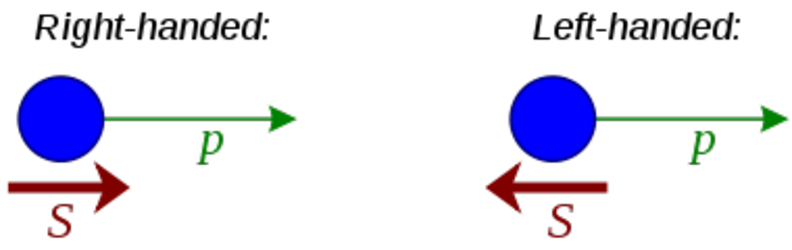
\includegraphics[scale=0.8]{figures/380px-Right_left_helicity.pdf}
%This figure is from http://commons.wikimedia.org/wiki/File:Right_left_helicity.svg
\caption{Helicity. In the left hand side, the spin and momentum are parallel (helicity $+1$); in the right hand side they are antiparallel (helicity $-1$). Figure adapted from \url{http://commons.wikimedia.org/wiki/File:Right\_left\_helicity.svg}.}
\label{fig: helicity}
\end{figure}
Although helicity is invariant under rotations, it is not invariant under boosts.
The only exception is when particles are massless, the helicity is Lorentz invariant because massless particles would move at the speed of light.

The chirality is related to the matrix $\gamma_{5}$ which is defined as
\begin{equation}
\gamma_{5} = \gamma^{5} \equiv i \gamma^{0} \gamma^{1} \gamma^{2} \gamma^{3}
\end{equation}
and has the following properties
\begin{equation}
\{ \gamma_{5}, \gamma_{\mu} \} = 0, \quad 
\gamma_{5}^{\dagger} = \gamma_{5}, \quad 
(\gamma_{5})^{2} = 1
\end{equation}
The chirality operators are defined as
\begin{equation}
P_{L} = \frac{1 - \gamma_{5}}{2}, \quad 
P_{R} = \frac{1 + \gamma_{5}}{2}
\end{equation}
A particle bi-spinor $\psi$ is consist of a left-chiral and a right-chiral part,
\begin{equation}
\psi = \psi_{L} + \psi_{R}
\end{equation}
where
\begin{equation}
\psi_{L} = P_{L} \psi, \quad 
\psi_{R} = P_{R} \psi
\end{equation}
It is obviously to show that $P_{L} \psi_{R} = 0$ and $P_{R} \psi_{L} = 0$.
The chirality of the field has the property that a left-chiral solution of the Dirac equation remains left-chiral under Lorentz transformation and same for right-chiral field.
Since $\gamma_{5}$ anticommutes with all the other $\gamma$ matrices, the chirality is not conserved because of the mass term in the Dirac Hamiltonian $H = \gamma^{0} (\gamma^{i} p_{i} + m)$.
If we are talking about massless particles, the difference between helicity and chirality disappear.
The relation between helicity and chirality for massless particles can be found in \cite{arXiv:1006.1718v2}.



\section{Grassmann numbers}
The Grassmann numbers are anticommuting objects
\begin{equation}
\{\theta_{\alpha}, \theta_{\beta}\} = \{\overline{\theta}_{\dot{\alpha}}, \overline{\theta}_{\dot{\beta}}\} = \{\theta_{\alpha}, \overline{\theta}_{\dot{\beta}}\} = 0
\end{equation}
where $\alpha, \beta, \dot{\alpha}$, and $\dot{\beta} = 1, 2$.
We can easily prove the following identities:
\begin{align}
&\theta_{\alpha} \theta_{\beta} = \frac{1}{2} \epsilon_{\alpha \beta} \theta \theta, \quad 
\overline{\theta}_{\dot{\alpha}} \overline{\theta}_{\dot{\beta}} = -\frac{1}{2} \epsilon_{\dot{\alpha} \dot{\beta}} \overline{\theta} \overline{\theta}, \quad 
\theta_{\alpha} \overline{\theta}_{\dot{\beta}} = \frac{1}{2} \sigma^{\mu}_{\alpha \dot{\beta}} (\overline{\theta} \overline{\sigma}_{\mu} \theta) \notag \\
& (\theta \psi)(\theta \chi) = - \frac{1}{2}\theta \theta \psi \chi, \quad 
(\overline{\theta} \overline{\psi})(\overline{\theta} \overline{\chi}) = - \frac{1}{2} \overline{\theta} \overline{\theta} \overline{\psi} \overline{\chi}, \quad 
(\theta \psi)(\overline{\theta} \overline{\chi}) = \frac{1}{2}(\overline{\theta} \overline{\sigma}^{\mu} \theta)(\psi \sigma_{\mu} \overline{\chi}) \notag \\
& (\theta \sigma^{\mu} \overline{\theta})(\theta \sigma^{\nu} \overline{\theta}) = \frac{1}{2} \theta \theta \overline{\theta} \overline{\theta} g^{\mu \nu} .
\end{align}
Derivatives with respect to the Grassmann numbers are defined by
\begin{equation}
\frac{\partial}{\partial \theta^{\alpha}}(\theta^{\beta}) = \delta^{\beta}_{\alpha}, \quad
\frac{\partial}{\partial \overline{\theta}_{\dot{\alpha}}}(\overline{\theta}_{\dot{\beta}}) = \delta^{\dot{\alpha}}_{\dot{\beta}}, \quad 
\frac{\partial}{\partial \theta^{\alpha}}(\overline{\theta}_{\dot{\beta}}) = 0, \quad 
\frac{\partial}{\partial \overline{\theta}_{\dot{\alpha}}}(\theta^{\beta}) = 0
\end{equation}
and the integrations are defined as
\begin{equation}
\int d\theta_{\alpha} = 0, \quad 
\int d\theta_{\alpha} \ \theta_{\alpha}  = 1 .
\end{equation}
If we have a general function $f$ which is linear in $\theta_{\alpha}$:
\begin{equation}
f(\theta_{\alpha}) = f_{0} + \theta_{\alpha} f_{1} ,
\end{equation}
where $f_{0}$ and $f_{1}$ can be functions of other commuting or anticommuting variables but not functions of $\theta_{\alpha}$.
We can find the differentiation and integration get the same results for Grassmann numbers
\begin{equation}
\frac{df}{d\theta_{\alpha}} = f_{1}, \quad \int d\theta_{\alpha} f(\theta_{\alpha}) = f_{1} .
\end{equation}
We also define
\begin{equation}
d^{2} \theta = \frac{1}{2} d\theta^{1} d\theta^{2}, \quad  
d^{2}\overline{\theta} = \frac{1}{2} d\overline{\theta}^{2} d\overline{\theta}^{1} = (d^{2} \theta)^{\dag}
\end{equation}
such that
\begin{equation}
\int d^{2} \theta \ \theta \theta = \int d^{2} \overline{\theta} \ \overline{\theta} \overline{\theta} = 1 .
\end{equation}



\section{Supermultiplets} \label{sec: supermultiplets}
The enlarged Poincar\'{e} group, called super-Poincar\'{e}, has generators $Q^{I}_{\alpha}$ and its conjugate $\overline{Q}^{I}_{\dot{\alpha}}$ which obey the commutation relations
\begin{align}
& [P_{\mu}, Q^{I}_{\alpha}] = 0, \quad 
[P_{\mu}, \overline{Q}^{I}_{\dot{\alpha}}] = 0,\\
& [M_{\mu \nu}, Q^{I}_{\alpha}] = i {(\sigma_{\mu \nu})_{\alpha}}^{\beta} Q^{I}_{\beta}, \quad 
[M_{\mu \nu}, \overline{Q}^{I\dot{\alpha}}] = i {(\overline{\sigma}_{\mu \nu})^{\dot{\alpha}}}_{\dot{\beta}} \overline{Q}^{I \dot{\beta}}\\
& \{Q^{I}_{\alpha}, \overline{Q}^{J}_{\dot{\beta}}\} = 2 \sigma^{\mu}_{\alpha \dot{\beta}} P_{\mu} \delta^{IJ}\\
& \{Q^{I}_{\alpha}, Q^{J}_{\beta}\} = \epsilon_{\alpha \beta} Z^{IJ}, \quad 
\{\overline{Q}^{I}_{\dot{\alpha}}, \overline{Q}^{J}_{\dot{\beta}}\} = \epsilon_{\dot{\alpha} \dot{\beta}} (Z^{IJ})^{*}
\end{align}
where $I, J = 1, \dots, N$ and the central charge $Z^{IJ} = -Z^{JI}$ is non vanish only for $N > 1$ and commutes with all generators.
Although there is no limit on $N$ from algebraic point of view, $N$ must less or equal than $8$ in order to have physical meaning.
We only discuss the simplest case $N = 1$ and do not talk about the extended SUSY ($N > 1$ case).

From the commutation relations listed above, it is easy to show that $[J_{3}, Q^{I}_{1}] = \frac{1}{2} Q^{I}_{1}$ and $[J_{3}, Q^{I}_{2}] = - \frac{1}{2} Q^{I}_{2}$.
Similarly, $[J_{3}, (Q^{I}_{1})^{\dag}] = -\frac{1}{2} (Q^{I}_{1})^{\dag}$ and $[J_{3}, (Q^{I}_{2})^{\dag}] = \frac{1}{2} (Q^{I}_{2})^{\dag}$.
Hence we can conclude that $Q^{I}_{1}$ and $(Q^{I}_{2})^{\dag}$ rise the z-component of the spin (helicity) by $\frac{1}{2}$ and $Q^{I}_{2}$ and $(Q^{I}_{1})^{\dag}$ lower it by $\frac{1}{2}$.

The single particle states of a SUSY theory correspond to a irreducible representations of super-Poincar\'{e} algebra, called supermultiplets.
Every supermultiplet contains both bosons and fermions with equal number of degrees of freedom and all particles belong to the same supermultiplet have the same mass because $P^{2}$ commutes with all generators of the SUSY algebra.
If we consider a massless supermultiplet in unextended SUSY ($N = 1$), there three kinds of multiplets:
$(0, \frac{1}{2}) \otimes (-\frac{1}{2}, 0)$, the chiral multiplet, which contains a complex scalar and a Weyl fermion;
$(\frac{1}{2}, 1) \otimes (-1, -\frac{1}{2})$, the vector multiplet, which contains a gauge boson and a Weyl fermion;
$(\frac{3}{2}, 2) \otimes (-2, -\frac{3}{2})$, the graviton multiplet, which contains a graviton and a gravitino.

For a massive case, there are 4 states: $(-\frac{1}{2}, 0, 0, \frac{1}{2})$ and the same for its CPT conjugate and $(-1, -\frac{1}{2}, -\frac{1}{2}, 0)$ and its CPT conjugate $(1, \frac{1}{2}, \frac{1}{2}, 0)$.
The detail discussions about massless and massive supermultiplets can be found in many materials such as \cite{Bilal} and \cite{larsenf}.





%%%%%
%%%%%
%%%%%
\chapter{The Wess-Zumino model}



\section{Supersymmetry transformation}
If the equation of motion is invariant under a transformation, we call this is a \textit{symmetry transformation}.
In other words, the action $S = \int d^{4}x \mathcal{L}$ is invariant under symmetry transformation.
There are two ways to keep the action S invariant: the Lagrangian $\mathcal{L}$ is either invariant or changes by a total derivative $\mathcal{L} \to \mathcal{L}' = \mathcal{L} + \partial_{\mu} \Lambda^{\mu}$ where we assume the quantity $\Lambda^{\mu}$ vanishes at the boundary.

Let us consider a Lagrangian
\begin{equation}
\mathcal{L} = \frac{1}{2} (\partial_{\mu} A)^{2} + \frac{1}{2} (\partial_{\mu} B)^{2} + \frac{i}{2} \overline{\psi} \ \slashed{\partial} \psi + \frac{1}{2} (F^{2} + G^{2})
\end{equation}
where $A, B, F$, and $G$ are real scalar fields and $\psi$ is 4-component a Majorana spinor field.
Wess and Zumino \cite{wess_and_zumino} defined an infinitesimal \textit{supersymmetry transformation}\footnote{It was called \textit{supergauge transformation} in the original paper written by Wess and Zumino.} by
\begin{align}
\delta A &= i \overline{\alpha} \gamma_{5} \psi ,\label{eq: 3.2}\\
\delta B &= - \overline{\alpha} \psi ,\\
\delta \psi &= -F \alpha + i G \gamma_{5} \alpha + \slashed{\partial} \gamma_{5} A \alpha + i \slashed{\partial} B \alpha ,\\
\delta F &= i \overline{\alpha} \slashed{\partial} \psi ,\\
\delta G &= \overline{\alpha} \gamma_{5} \slashed{\partial} \psi \label{eq: 3.6},
\end{align}
where the parameter $\alpha$ is an infinitesimal spinor which anticommutes with itself and with $\psi$ and commutes with the other fields.
Although the Lagrangian is not itself invariant, it changes by a total derivative under a supersymmetry transformation providing an invariant action.

We usually use complex fields $\mathcal{S}, \psi_{L}$ and $\mathcal{F}$ to replace the scalar fields and Majorana spinor field in Lagrangian
\begin{equation}
\mathcal{S} = \frac{1}{\sqrt{2}} (A + i B), \quad \psi_{L} = \frac{1 - \gamma_{5}}{2} \psi, \quad \mathcal{F} = \frac{1}{\sqrt{2}} (F + i G)
\end{equation}
then the SUSY transformations become
\begin{align}
\delta \mathcal{S} &= -i \sqrt{2} \overline{\alpha} \psi_{L} \label{eq: SUSY transformation 1}\\
\delta \psi_{L} &= - \sqrt{2} \mathcal{F} \alpha_{L} + \sqrt{2} \slashed{\partial} \mathcal{S} \alpha_{R} \label{eq: SUSY transformation 2}\\
\delta \mathcal{F} &= i \sqrt{2} \overline{\alpha} \slashed{\partial} \psi_{L} \label{eq: SUSY transformation 3} .
\end{align}
Thus, $\mathcal{S}, \psi_{L}$ and $\mathcal{F}$ transform into one another under the SUSY transformations.

The simplest example of a supersymmetric theory in four dimensions consists of a massless complex scalar field $\phi$ and its superpartner which is a massless left-handed two-component Weyl fermion $\psi$ without interactions between fields.
We can write down the simplest action immediately
\begin{align}
S &= \int d^{4} x \ (\mathcal{L}_{\mathrm{scalar}} + \mathcal{L}_{\mathrm{fermion}})\\
\mathcal{L}_{\mathrm{scalar}} &= \partial^{\mu} \phi^{*} \partial_{\mu} \phi, \quad \mathcal{L}_{\mathrm{fermion}} = i \psi^{\dag} \overline{\sigma}^{\mu} \partial_{\mu} \psi .
\end{align}
A SUSY transformation changes a boson field $\phi$ into fermions field $\psi$ so the simplest infinitesimal transformation of the scalar fields is
\begin{equation} \label{eq: susy transformation for boson fields}
\delta \phi  = \epsilon \psi, \quad \delta \phi^{*} = \epsilon^{\dag} \psi^{\dag} ,
\end{equation}
where $\epsilon^{\alpha}$ is a constant, infinitesimal, anticommuting, two-component object with mass dimension $-\frac{1}{2}$.
Similarly, a fermion field is turned into a scalar field under SUSY transformation
\begin{equation} \label{eq: susy transformation for fermion fields}
\delta \psi_{\alpha} = -i (\sigma^{\mu} \epsilon^{\dag})_{\alpha} \partial_{\mu} \phi, \quad \delta \psi^{\dag}_{\dot{\alpha}} = i (\epsilon \sigma^{\mu})_{\dot{\alpha}} \partial_{\mu} \phi^{*} .
\end{equation}
We can obtain the same transformation using equations (\ref{eq: 3.2}) to (\ref{eq: 3.6}) by setting $B = F = G =0$ and replacing $A \to \sqrt{2} \phi$ and $\psi \to \sqrt{2} \psi$ with suitable choose of $\epsilon$.
The variations of the scalar and fermion Lagrangian are
\begin{align}
\delta \mathcal{L}_{\mathrm{scalar}} &= \partial^{\mu} (\delta \phi^{*}) \partial_{\mu} \phi + \partial^{\mu} \phi^{*} \partial_{\mu} (\delta \phi) \notag \\
&= \epsilon \partial^{\mu} \psi \partial_{\mu} \phi^{*} + \epsilon^{\dag} \partial^{\mu} \psi^{\dag} \partial_{\mu} \phi\\
%
\delta \mathcal{L}_{\mathrm{fermion}} &= i (\delta \psi^{\dag}) \overline{\sigma}^{\mu} \partial_{\mu} \psi + i \psi^{\dag} \overline{\sigma}^{\mu} \partial_{\mu} (\delta \psi) \notag \\
&= -\epsilon \sigma^{\nu} \partial_{\nu} \phi^{*} \overline{\sigma}^{\mu} \partial_{\mu} \psi + \psi^{\dag} \overline{\sigma}^{\mu} \sigma^{\nu} \epsilon^{\dag} \partial_{\mu} \partial_{\nu} \phi \notag \\
&= -\epsilon \partial^{\mu} \partial_{\mu} \phi^{*} - \epsilon^{\dag} \partial^{\mu} \psi^{\dag} \partial_{\mu} \phi
+\partial_{\mu} (\epsilon \sigma^{\mu} \overline{\sigma}^{\nu} \psi \partial_{\nu} \phi^{*} - \epsilon \psi \partial^{\mu} \phi^{*} + \epsilon^{\dag} \psi^{\dag} \partial^{\mu}\phi) .
\end{align}
The sum of $\delta \mathcal{L}_{\mathrm{scalar}}$ and $\delta \mathcal{L}_{\mathrm{fermion}}$ gives a total derivative so the action is invariant.
Besides showing the action is invariant under SUSY transformation, we also need to show the SUSY algebra closes.
However, (\ref{eq: susy transformation for boson fields}) and (\ref{eq: susy transformation for fermion fields}) only valid for on-shell (i.e. $\overline{\sigma}^{\mu} \partial_{\mu} \psi = 0$).
We have to introduce a new complex scalar field $F$, called auxiliary field, with mass dimension 2 and it transform under SUSY as
\begin{equation}
\delta F = - i \epsilon^{\dag} \overline{\sigma}^{\mu} \partial_{\mu} \psi, \quad 
\delta F^{*} = i \partial_{\mu} \psi^{\dag} \overline{\sigma}^{\mu} \epsilon
\end{equation}
and (\ref{eq: susy transformation for fermion fields}) has to be modify to
\begin{equation}
\delta \psi_{\alpha} = -i (\sigma^{\mu} \epsilon^{\dag})_{\alpha} \partial_{\mu} \phi + \epsilon_{\alpha} F, \quad 
\delta \psi^{\dag}_{\dot{\alpha}} = i (\epsilon \sigma^{\mu})_{\dot{\alpha}} \partial_{\mu} \phi^{*} + \epsilon^{\dag}_{\dot{\alpha}} F^{*}.
\end{equation}
Then we can show that fields $X = \phi, \phi^{*}, \psi, \psi^{\dag}, F, F^{*}$ satisfy
\begin{equation}
(\delta_{\epsilon2} \delta_{\epsilon1} - \delta_{\epsilon1} \delta_{\epsilon2}) X = i (- \epsilon_{1} \sigma^{\mu} \epsilon^{\dag}_{2} + \epsilon_{2} \sigma^{\mu} \epsilon^{\dag}_{1}) \partial_{\mu} X
\end{equation}
and keep the Lagrangian $\mathcal{L} = \mathcal{L}_{\mathrm{scalar}} + \mathcal{L}_{\mathrm{fermion}} + \mathcal{L}_{\mathrm{auxiliary}}$ still invariant under SUSY transformation for off-shell case where the Lagrangian of auxiliary field is defined as $\mathcal{L}_{\mathrm{auxiliary}} = F^{*} F$.

Since SUSY is a kind of symmetry, we can find the conserved supercurrents and construct the conserved supercharges from Noether's theorem
\begin{align}
& J^{\mu}_{\alpha} = (\sigma^{\nu} \overline{\sigma}^{\mu} \psi)_{\alpha} \partial_{\nu} \phi^{*}, \quad 
J^{\dag \mu}_{\dot{\alpha}} = ( \psi^{\dag} \overline{\sigma}^{\mu} \sigma^{\nu})_{\dot{\alpha}} \partial_{\nu} \phi\\
%
& Q_{\alpha} = \sqrt{2} \int d^{3}x \ J^{0}_{\alpha}, \quad 
Q^{\dag}_{\dot{\alpha}} = \sqrt{2} \int d^{3}x J^{\dag 0}_{\dot{\alpha}} .
\end{align}
The supercharges play the role of generators of SUSY transformations and obey the commutation relations mentioned in section \ref{sec: supermultiplets}.



\section{Supersymmetric Lagrangian with interactions}
We have considered the free Lagrangian
\begin{equation} \label{eq: free Lagrangian}
\mathcal{L}_{\mathrm{free}} = \partial^{\mu} \phi^{*i} \partial_{\mu} \phi_{i} + i \psi^{\dag i} \overline{\sigma}^{\mu} \partial_{\mu} \psi_{i} + F^{*i} F_{i}
\end{equation}
and now let us consider the realistic theory which contains the interactions between fields.
The general non-gauge interaction Lagrangian for chiral supermultiplets can be written as
\begin{equation} \label{eq: non-gauge interaction Lagrangian}
\mathcal{L}_{\mathrm{int}} = \Big( - \frac{1}{2} W^{ij} \psi_{i} \psi_{j} + W^{i} F_{i}\Big) + \mathrm{c.c}
\end{equation}
where
\begin{equation}
W = \frac{1}{2} M^{ij} \phi_{i} \phi_{j} + \frac{1}{6} y^{ijk} \phi_{i} \phi_{j} \phi_{k}
\end{equation}
is the superpotential and $W^{i}$ is defined as 
\begin{equation}
W^{i} \equiv \frac{\partial W}{\partial \phi_{i}} = M^{ij} \phi_{j} + \frac{1}{2} y^{ijk} \phi_{j} \phi_{k}.
\end{equation}
The auxiliary fields $F_{i}$ and $F^{*i}$ can be replaced using equations of motion.
From (\ref{eq: free Lagrangian}) and (\ref{eq: non-gauge interaction Lagrangian}), we find the part of the $\mathcal{L}_{\mathrm{free}} + \mathcal{L}_{\mathrm{int}}$ contains the auxiliary fields is $F^{*i} F_{i} + W^{i} F_{i} + W^{*}_{i} F^{*i}$, leading to the equations of motion
\begin{equation} \label{eq: auxiliary field F}
F_{i} = - W^{*}_{i}, \quad 
F^{*i} = - W^{i} .
\end{equation}
Thus the Lagrangian becomes
\begin{align} \label{eq: Lagrangian with interaction}
\mathcal{L} &= \mathcal{L}_{\mathrm{free}} + \mathcal{L}_{\mathrm{int}} \notag \\
&= \partial^{\mu} \phi^{*i} \partial_{\mu} \phi_{i} + i \psi^{\dag i} \overline{\sigma}^{\mu} \partial_{\mu} \psi_{i} -\frac{1}{2} \Big( W^{ij} \psi_{i} \psi_{j} + W^{*}_{ij} \psi^{\dag i} \psi^{\dag j} \Big) - W^{i} W^{*}_{i} .
\end{align}
From equations (\ref{eq: auxiliary field F}) and (\ref{eq: Lagrangian with interaction}), we know the scalar potential is given in terms of superpotential by
\begin{equation}
V(\phi, \phi^{*}) = W^{i}W^{*}_{i} = F^{*i} F_{i}
\end{equation}
which is non-negative.


%%%%%
%%%%%
%%%%%
\chapter{Superspace and superfields}
The supersymmetric formalism can be recast in an elegant way by introducing superspace and superfields.
A superspace is described by the four ordinary space-time coordinates $x^{\mu}$ and four anticommuting Grassmannian coordinates $\theta_{\alpha}$ and $\overline{\theta}_{\dot{\alpha}}$, where the spinor indices $\alpha = 1, 2$ and $\dot{\alpha} = 1, 2$.
A superfield is a function of superspace coordinates: $S (x^{\mu}, \theta_{\alpha}, \overline{\theta}_{\dot{\alpha}})$, which contains bosonic, fermonic and auxiliary fields in the corresponding supermultiplet.



\section{Superspace}
Since $\theta_{\alpha}$ and $\overline{\theta}_{\dot{\alpha}}$ anticommute among themselves, any product cannot contain more than two $\theta$'s or more than two $\overline{\theta}$'s.
A general superfield can be expanded in terms of $\theta$ and $\overline{\theta}$
\begin{equation}
S(x, \theta, \overline{\theta}) = a + \theta \xi + \overline{\theta} \overline{\chi} + \theta \theta b + \overline{\theta} \overline{\theta} c + \overline{\theta} \overline{\sigma}^{\mu} \theta v_{\mu} + \theta \theta \overline{\theta} \overline{\zeta} + \overline{\theta} \overline{\theta} \theta \eta + \theta \theta \overline{\theta} \overline{\theta} d
\end{equation}
The 8 bosonic component fields $a, b, c, d$, and $v_{\mu}$ and 4 two-component fermion component fields $\xi, \overline{\chi}, \eta, \overline{\zeta}$ are complex functions of $x^{\mu}$.
To formulate SUSY transformation in superspace, we define the SUSY generators 
\footnote{We also can define 
$Q^{\alpha} = i \frac{\partial}{\partial \theta_{\alpha}} + (\overline{\theta} \overline{\sigma}^{\mu})^{\alpha} \partial_{\mu}$ and 
$\overline{Q}^{\dot{\alpha}} = -i \frac{\partial}{\partial \overline{\theta}_{\dot{\alpha}}} - (\overline{\sigma}^{\mu} \theta)^{\dot{\alpha}} \partial_{\mu}$}
\begin{equation}
Q_{\alpha} = -i \frac{\partial}{\partial \theta^{\alpha}} - \sigma^{\mu}_{\alpha \dot{\beta}} \overline{\theta}^{\dot{\beta}} \partial_{\mu}, \quad 
\overline{Q}_{\dot{\alpha}} = i \frac{\partial}{\partial \overline{\theta}^{\dot{\alpha}}} + \theta^{\beta} \sigma^{\mu}_{\beta \dot{\alpha}} \partial_{\mu}
\end{equation}
and they follow the commutation relations
\begin{align}
& \{Q_{\alpha}, \overline{Q}_{\dot{\beta}}\} = 2 \sigma^{\mu}_{\alpha \dot{\beta}} P_{\mu} = -2i \sigma^{\mu}_{\alpha \dot{\beta}} \partial_{\mu} \\
& \{Q_{\alpha}, Q_{\beta}\} = 0, \quad 
\{\overline{Q}_{\dot{\alpha}}, \overline{Q}_{\dot{\beta}}\} = 0 .
\end{align}
Then the infinitesimal SUSY transformation can be written as
\begin{align}
\delta_{\epsilon} S(x, \theta, \overline{\theta}) &= S(x^{\mu} + i \epsilon \sigma^{\mu}\overline{\theta} + i \overline{\epsilon} \overline{\sigma}^{\mu} \theta, \theta + \epsilon, \overline{\theta} + \overline{\epsilon}) - S(x, \theta, \overline{\theta})\\
&= (i \epsilon Q + i \overline{\epsilon} \overline{Q}) S(x, \theta, \overline{\theta})\\
&= \Big[ \epsilon^{\alpha} \frac{\partial}{\partial \theta^{\alpha}} + \overline{\epsilon}_{\dot{\alpha}} \frac{\partial}{\partial \overline{\theta}_{\dot{\alpha}}} - i \big( \epsilon \sigma^{\mu} \overline{\theta} + \overline{\epsilon} \overline{\sigma}^{\mu} \theta \big)  \Big] S(x, \theta, \overline{\theta})
\end{align}
Now we introduce SUSY covariant derivatives $D_{\alpha}$ and $\overline{D}_{\dot{\alpha}}$ that anticommute with SUSY generators $Q$ and $\overline{Q}$
\begin{equation}
D_{\alpha} = \frac{\partial}{\partial \theta^{\alpha}} + i \sigma^{\mu}_{\alpha \dot{\beta}} \overline{\theta}^{\dot{\beta}} \partial_{\mu}, \quad 
\overline{D}_{\dot{\alpha}} = (D_{\alpha})^{\dag} = \frac{\partial}{\partial \overline{\theta}^{\dot{\alpha}}} + i \theta^{\beta} \sigma^{\mu}_{\beta \dot{\alpha}} \partial_{\mu}
\end{equation}
with the commutation relations
\begin{align*}
& \{ D_{\alpha}, \overline{D}_{\dot{\beta}}\} = 2i \sigma^{\mu}_{\alpha \dot{\beta}} \partial_{\mu}, \quad \{ D_{\alpha}, D_{\beta}\} = \{ \overline{D}_{\dot{\alpha}}, \overline{D}_{\dot{\beta}}\} = 0\\
& \{ D_{\alpha}, Q_{\beta} \} = \{ D_{\alpha}, \overline{Q}_{\dot{\beta}}\} = \{ \overline{D}_{\dot{\alpha}}, Q_{\beta} \} = \{ \overline{D}_{\dot{\alpha}}, \overline{Q}_{\dot{\beta}}\} = 0  
\end{align*}
Then we can find $\delta_{\epsilon} (D_{\alpha} S) = D_{\alpha} (\delta_{\epsilon} S)$ and $\delta_{\epsilon} (\overline{D}_{\dot{\alpha}} S) = \overline{D}_{\dot{\alpha}} (\delta_{\epsilon} S)$.



\section{Chiral superfields}
The chiral superfields, which are irreducible representations of the SUSY algebra, can describe spin 0 bosons and spin 1/2 fermions, for example, the Higgs boson and the quarks and leptons.
A superfield $\Phi (x, \theta, \overline{\theta})$ satisfies the condition
\begin{equation} \label{eq: definition of chiral superfield}
\overline{D}_{\dot{\alpha}} \Phi =0
\end{equation}
 is called a chiral (or left-chiral) superfield and its complex conjugate $\Phi^{*}$ is called antichiral (or right-chiral) superfield and satisfies
 \begin{equation} \label{eq: definition of antichiral superfield}
D_{\alpha} \Phi^{*} = 0.
\end{equation}
It is convenient to define the chiral coordinates $(y^{\mu}, \theta)$ and antichiral coordinates $(\overline{y}^{\mu}, \overline{\theta})$, where
\begin{equation}
y^{\mu} = x^{\mu} + i \theta \sigma^{\mu} \overline{\theta}, \quad 
\overline{y}^{\mu} = x^{\mu} - i \theta \sigma^{\mu} \overline{\theta}
\end{equation}
and the covariant derivative in (anti)chiral coordinates becomes
\begin{equation}
D_{\alpha} = \frac{\partial}{\partial \theta^{\alpha}} + 2 i \sigma^{\mu}_{\alpha \dot{\beta}} \overline{\theta}^{\dot{\beta}} \frac{\partial}{\partial y^{\mu}}, \quad 
\overline{D}_{\dot{\alpha}} = \frac{\partial}{\partial \overline{\theta}^{\dot{\alpha}}} .
\end{equation}
Now the general form of a chiral superfield is a function of $y^{\mu}$ and $\theta$ only and can be expanded as
\begin{equation}
\Phi (y, \theta) = \phi (y) + \sqrt{2} \theta \psi (y) + \theta \theta F(y) .
\end{equation}
By using $\delta_{\epsilon} \Phi = (i \epsilon Q + i \overline{\epsilon} \overline{Q}) \Phi$, we can get the SUSY transformations of the component fields
\begin{align} 
\delta_{\epsilon} \phi &= \sqrt{2} \epsilon \psi \label{eq: SUSY transformation 4}\\
\delta_{\epsilon} \psi_{\alpha} &= i \sqrt{2}  \partial_{\mu} \phi (\sigma^{\mu} \overline{\epsilon})_{\alpha} - \sqrt{2} \epsilon_{\alpha} F \label{eq: SUSY transformation 5}\\
\delta_{\epsilon} F &= i \sqrt{2}  \partial_{\mu} \psi \sigma^{\mu} \overline{\epsilon} \label{eq: SUSY transformation 6}
\end{align}
in agreement with equations (\ref{eq: SUSY transformation 1}), (\ref{eq: SUSY transformation 2}), and (\ref{eq: SUSY transformation 3}), up to a multiplicative.



\section{Vector superfields}
In order to describe the spin 1 gauge bosons, we have to introduce the vector (real) superfields $V$ which are defined as
\begin{equation}
V(x, \theta, \overline{\theta}) = V^{\dag} (x, \theta, \overline{\theta}) .
\end{equation}
The general vector superfield $V(x, \theta, \overline{\theta})$ has the expansion
\begin{align}
V(x, \theta, \overline{\theta}) &= C + i \theta \chi - i \overline{\theta} \overline{\chi} + \theta \sigma^{\mu} \overline{\theta} v_{\mu} + \frac{i}{2} \theta \theta (M + iN) - \frac{i}{2} \overline{\theta} \overline{\theta} (M - iN) \notag \\
& + i \theta \theta \overline{\theta} (\overline{\lambda} + \frac{i}{2} \overline{\sigma}^{\mu} \partial_{\mu} \chi ) - i \overline{\theta} \overline{\theta} \theta (\lambda - \frac{i}{2} \sigma^{\mu} \partial_{\mu} \overline{\chi}) + \frac{1}{2} \theta \theta \overline{\theta} \overline{\theta} (D - \frac{1}{2} \partial^{2} C)
\end{align}
where $C, M, N$, and $D$ are real scalars, $\chi$ and $\lambda$ are Weyl spinors, and $v^{\mu}$ is a vector field.
Since there are too many component fields in a single supermultiplet, we want to reduce the number of them.
Consider an abelian SUSY gauge transformation for a vector superfield
\begin{equation}
V \to V + i (\Lambda - \Lambda^{\dag})
\end{equation}
where the gauge transformation parameter $\Lambda$ is a chiral superfield. Then the components fields $C, \chi, M, N$ and one component of $v_{\mu}$ can be gauged away.
This is called Wess-Zumino gauge.
By introducing Wess-Zumino gauge, we can reduce the number of components of the vector superfield as
\begin{equation} \label{eq: WZ gauge vector superfield}
V_{WZ} = \theta \sigma^{\mu} \overline{\theta} v_{\mu}(x) + i \theta \theta \overline{\theta} \overline{\lambda}(x) - i \overline{\theta} \overline{\theta} \theta \lambda(x) + \frac{1}{2} \theta \theta \overline{\theta} \overline{\theta} D(x) .
\end{equation}
Since there are at least one $\theta$ in the $V_{WZ}$, the only non-vanishing power of $V_{WZ}$ is
\begin{equation}
V^{2}_{WZ} = \big[ \theta \sigma^{\mu} \overline{\theta} v_{\mu}(x) \big] \big[ \theta \sigma^{\nu} \overline{\theta} v_{\nu}(x) \big] = \frac{1}{2} \theta \theta \overline{\theta} \overline{\theta} v_{\mu} v^{\mu}
\end{equation}
and $V^{n}_{WZ} = 0, n \ge 3$.




%%%%%
%%%%%
%%%%%
\chapter{Supersymmetric gauge theories}

Since all the known interactions are gauge interactions, we have to extend gauge interactions to its supersymmetric version.
This can be divided into two cases, one for Ableian and one for non-Abelian.



\section{Lagrangians for gauge superfields}
A vector superfield V which is used to describe the gauge bosons contains a massless gauge boson field $A^{a}_{\mu}$ \footnote{The field $A^{\mu}$ is defined as $(V, \vec{A})$ which is the conventions in electrodynamics.} and a gaugino field $\lambda^{a}$.
Under the gauge transformation, they transform as
\begin{align}
& A^{a}_{\mu} \to A^{a}_{\mu} + \partial_{\mu} \Lambda^{a} + g f^{abc} A^{b}_{\mu} \Lambda^{c} ,\\
& \lambda^{a} \to \lambda^{a} + g f^{abc} \lambda^{b} \Lambda^{c}
\end{align}
where $\Lambda^{a}$ is an infinitesimal gauge transformation parameter, $g$ is the gauge coupling, and $f^{abc}$ are the antisymmetric structure constants of the gauge group.
Because gauge transformation removes one degree of freedom from $A^{a}_{\mu}$, we have to introduce a real bosonic auxiliary field $D^{a}$.
This gauge auxiliary field has mass dimension 2 and no kinetic term, so it can be eliminated using equation of motion.
The Lagrangian density of a gauge superfields is
\begin{equation} \label{eq: L_gauge}
\mathcal{L}_{\mathrm{gauge}} = - \frac{1}{4} F^{a}_{\mu \nu} F^{\mu \nu a} + i \lambda^{\dag a} \overline{\sigma}^{\mu} \nabla_{\mu} \lambda^{a} + \frac{1}{2} D^{a} D^{a} ,
\end{equation}
where
\begin{equation} \label{eq: gauge field strength}
F^{a}_{\mu \nu} = \partial_{\mu} A^{a}_{\nu} - \partial_{\nu} A^{a}_{\mu} + g f^{abc} A^{b}_{\mu} A^{c}_{\nu}
\end{equation}
is the gauge field strength and
\begin{equation}
\nabla_{\mu} \lambda^{a} = \partial_{\mu} \lambda^{a} + g f^{abc} A^{b}_{\mu} \lambda^{c}
\end{equation}
is the covariant derivative of the gaugino field.
If we apply SUSY transformation to the fields $A^{a}_{\mu}$, $\lambda^{a}$, and $D^{a}$, we can find the $\mathcal{L}_{\mathrm{gauge}}$ is supersymmetric.



\section{Supersymmetric gauge interactions}
When gauge interactions are involved, we have to promote the ordinary derivative to a gauge-covariant derivative
\begin{equation}
\partial_{\mu} \psi_{i} \to \nabla_{\mu} \psi_{i} = \partial_{\mu} \psi_{i} - i g_{a} A^{a}_{\mu} T^{aj}_{i} \psi_{j}
\end{equation}
where $g_{a}$ is the gauge coupling, $T^{a}$ is the generator matrix, and $A^{a}_{\mu}$ is the vector field.
And the SUSY transformations are modified to
\begin{align} \label{eq: total Lagrangian}
\delta \phi_{i} &= \epsilon \psi_{i}\\
\delta (\psi_{i})_{\alpha} &= - i (\sigma^{\mu} \epsilon^{\dag})_{\alpha} \nabla_{\mu} \phi_{i} + \epsilon_{\alpha} F_{i}\\
\delta F_{i} &= -i \epsilon^{\dag} \overline{\sigma}^{\mu} \nabla_{\mu} \psi_{i} + \sqrt{2} g (T^{a} \phi)_{i} \epsilon^{\dag} \lambda^{\dag a}
\end{align}
With the help of the extra term $\sqrt{2} g (T^{a} \phi)_{i} \epsilon^{\dag} \lambda^{\dag a}$ in $\delta F_{i}$, the total Lagrangian density
\begin{align} \label{eq: Lagrangian for gauge theory}
\mathcal{L} &= \nabla^{\mu} \phi^{*i} \nabla_{\mu} \phi_{i} + i \psi^{\dag i} \overline{\sigma}^{\mu} \nabla_{\mu} \psi_{i} -\frac{1}{2} \Big( W^{ij} \psi_{i} \psi_{j} + W^{*}_{ij} \psi^{\dag i} \psi^{\dag j} \Big) - W^{i} W^{*}_{i} \notag \\
& -\frac{1}{4} F^{a}_{\mu \nu} F^{\mu \nu a} + i \lambda^{\dag a} \overline{\sigma}^{\mu} \nabla_{\mu} \lambda^{a} + \frac{1}{2} D^{a} D^{a} \notag \\
& -\sqrt{2} g (\phi^{*} T^{a} \psi) \lambda^{a} - \sqrt{2} g \lambda^{\dag a} (\psi^{\dag} T^{a} \phi) + g(\phi^{*} T^{a} \phi) D^{a}
\end{align}
is invariant under the SUSY transformations.
From this Lagrangian, we can combine the $D^{a} D^{a} / 2$ term with $g (\phi^{*} T^{a} \phi) D^{a}$ to find the equations of motion for auxiliary field $D^{a}$
\begin{equation} \label{eq: E.O.M of D field}
D^{a} = - g (\phi^{*} T^{a} \phi) .
\end{equation}
Replacing the auxiliary field in (\ref{eq: total Lagrangian}) using (\ref{eq: E.O.M of D field}), we can find the scalar potential is
\begin{equation} \label{eq: scalar potential}
V(\phi, \phi^{*}) = F^{*i} F_{i} + \frac{1}{2} \sum_{a} D^{a} D_{a} = W^{i} W^{*}_{i} + \frac{1}{2} \sum_{a} g^{2}_{a} (\phi^{*} T^{a} \phi)^{2} .
\end{equation}
Since $V(\phi, \phi^{*})$ is a sum of square terms, it is non-negative.



\section{Superspace Lagrangians for Abelian and non-Abelian gauge theory}
Although we have obtained the Lagrangian for Abelian gauge theory in (\ref{eq: Lagrangian for gauge theory}), there is another way to compute the Lagrangians using the gauge-invariant Abelian field strength superfields which is defined as
\begin{equation}
W_{\alpha} = -\frac{1}{4} \overline{D} \overline{D} D_{\alpha} V, \quad
\overline{W}_{\dot{\alpha}} = -\frac{1}{4} D D \overline{D}_{\dot{\alpha}}
\end{equation}
with mass dimension $3/2$.
Since $D^{3} = \overline{D}^{3} = 0$, from (\ref{eq: definition of chiral superfield}) and (\ref{eq: definition of antichiral superfield}) we know $W_{\alpha}$ is chiral and $\overline{W}_{\dot{\alpha}}$ is antichiral.
Because $W_{\alpha}$ is gauge invariant, the easiest way to derive the general expression is using the Wess-Zumino gauge.
After converting the vector superfields V in (\ref{eq: WZ gauge vector superfield}) to $(y^{\mu}, \theta_{\alpha}, \overline{\theta}_{\dot{\alpha}})$ coordinate, we get
\begin{equation}
V (y, \theta, \overline{\theta}) |_{\mathrm{WZ}} = \theta \sigma^{\mu} \overline{\theta} A_{\mu} (y) + i \theta \theta \overline{\theta} \overline{\lambda} (y) - i \overline{\theta} \overline{\theta} \theta \lambda (y) + \frac{1}{2} \theta \theta \overline{\theta} \overline{\theta} [ D(y) - i \partial_{\mu} A^{\mu} (y) ]
\end{equation}
and
\begin{equation} \label{eq: field strength chiral superfield in abelian gauge}
W_{\alpha} = -i \lambda_{\alpha} (y) + \theta_{\alpha} D(y) + \frac{i}{2} (\sigma^{\mu} \overline{\sigma}^{\nu} \theta)_{\alpha} F_{\mu \nu} (y) - i \theta \theta (\sigma^{\mu} \partial_{\mu} \overline{\lambda} (y))_{\alpha}
\end{equation}
where $F_{\mu \nu}$ is the field strength.
Since $W_{\alpha}$ is a chiral superfield, we can calculate the SUSY invariant Lagrangian
\begin{equation}
\mathcal{L} = \int d^{2} \theta \ \frac{1}{4} [W^{\alpha} W_{\alpha}] + c.c = \frac{1}{2} D^{2} + i \overline{\lambda} \overline{\sigma}^{\mu} \partial_{\mu} \lambda - \frac{1}{4} F^{\mu \nu} F_{\mu \nu}
\end{equation}
and agree with (\ref{eq: L_gauge}).

For a non-Abelian gauge group, the vector superfields transform as
\begin{align}
e^{V} &\to e^{i \Lambda^{\dag}} e^{V} e^{-i \Lambda}\\
e^{-V} & \to e^{i \Lambda} e^{-V} e^{-i \Lambda^{\dag}}
\end{align}
and the field strength chiral superfield becomes
\begin{equation}
W_{\alpha} = -\frac{1}{4} \overline{D} \overline{D} (e^{-V} D_{\alpha} e^{V})
\end{equation}
and it transforms under supergague transformations as
\begin{equation}
W_{\alpha} \to e^{i \Lambda} W_{\alpha} e^{-i \Lambda}.
\end{equation}
After applying Wess-Zumino gauge, the component expansion of $W_{\alpha}$ is
\begin{equation}
W_{\alpha} = -i \lambda_{\alpha} (y) + \theta_{\alpha} D(y) + \frac{i}{2} (\sigma^{\mu} \overline{\sigma}^{\nu} \theta)_{\alpha} F_{\mu \nu} (y) - i \theta \theta (\sigma^{\mu} \nabla_{\mu} \overline{\lambda} (y))_{\alpha}
\end{equation}
which is the same as (\ref{eq: field strength chiral superfield in abelian gauge}) except the ordinary derivatives of the field turn into gauge corivant derivatives and the gauge field strength $F_{\mu \nu}$ is defined in (\ref{eq: gauge field strength}).
If we introduce complex coupling constant
\begin{equation}
\tau = \frac{\Theta}{2 \pi} + \frac{4 \pi i}{g^{2}}
\end{equation}
where $g$ is the gauge coupling constant and $\Theta$ is $\Theta$-angle.
Then the general Lagrangian for supersymmetric gauge theory is
\begin{align}
\mathcal{L} &= \frac{1}{32 \pi} \Im (\tau \int d^{2} \theta \ \mathrm{Tr} W^{\alpha} W_{\alpha}) \notag\\
&= \mathrm{Tr} \big( -\frac{1}{4} F_{\mu \nu} F^{\mu \nu} -i \lambda \sigma^{\mu} D_{\mu} \overline{\lambda} + \frac{1}{2} D^{2} \big)
+ \frac{\Theta}{32 \pi^{2}} g^{2} \ \mathrm{Tr} F_{\mu \nu} \widetilde{F}^{\mu \nu}
\end{align}
where
\begin{equation}
\widetilde{F}^{\mu \nu} = \frac{1}{2} \epsilon^{\mu \nu \rho \sigma} F_{\rho \sigma}
\end{equation}
is the dual field strength.





%%%%%
%%%%%
%%%%%
\chapter{Supersymmetry breaking}

As mentioned in section \ref{sec: supermultiplets}, all particles belong to the same supermultiplet have the same mass.
That is to say, the mass of SM particles and their superpartners are identical.
However, it is not true in reality because we didn't find any sparticle, for example, there is no selectron with mass 0.51 MeV and a massless fermionic partner of photon.
Hence the supersymmetry must be spontaneously broken.



\section{Vacuum expectation value in SUSY}
The superalgebra tells us the anticommutation relation $\{ Q_{\alpha}, \overline{Q}_{\dot{\beta}} \} = 2 \sigma^{\mu}_{\alpha \dot{\beta}} P_{\mu}$.
So we have
\begin{align}
\{ Q_{1}, \overline{Q}_{1} \} = 2 ( P_{0} + P_{3}) \notag \\
\{ Q_{2}, \overline{Q}_{2} \} = 2 ( P_{0} - P_{3}) 
\end{align}
Then the Hamiltonian for SUSY is given by
\begin{equation}
H \equiv P^{0} = \frac{1}{4} (\{ Q_{1}, \overline{Q}_{1} \}  + \{ Q_{2}, \overline{Q}_{2} \} ) .
\end{equation}
It follows that the expectation value of the Hamiltonian for an arbitrary state $| \Psi \rangle$ is a sum of squares and therefore non-negative
\begin{equation}
E_{\Psi} = \langle \Psi | H | \Psi \rangle = \frac{1}{4} \sum_{\alpha} ( \| Q_{\alpha} | \Psi \rangle \|^2 + \| \overline{Q}_{\dot{\alpha}} | \Psi \rangle \|^2 ) \ge 0 .
\end{equation}
For a vacuum state (ground state) $|\Psi \rangle = | \Omega \rangle$, $E = 0$ if and only if $Q_{\alpha} | \Omega \rangle = \overline{Q}_{\dot{\alpha}} | \Omega \rangle = 0$.
If a ground state has non-vanishing positive energy, the SUSY is broken spontaneously. 



\section{The $F$-term breaking and $D$-term breaking}
A state $| \Omega \rangle$ is called a vacuum state when the scalar potential $V$ has a minimum.
There are two kinds of vacuum, the true vacuum and the false vacuum.
If the minimum of $V$ is the global minimum, then the vacuum is the true vacuum, otherwise it is a false vacuum.
The scalar potential is given in (\ref{eq: scalar potential})
\begin{equation}
V(\phi, \phi^{*}) = F^{*i} F_{i} + \frac{1}{2} \sum_{a} D^{a} D_{a} \notag
\end{equation}
and it is non-negative. 
It is clear that when $F_{i} = D_{a} = 0$ then $V = 0$ is a global minimum.

Consider the SUSY transformation (\ref{eq: SUSY transformation 4}), (\ref{eq: SUSY transformation 5}), (\ref{eq: SUSY transformation 6}), the SUSY is broken if one of $\delta \phi$, $\delta \psi$, $\delta F \neq 0$.
Since a vacuum state is Lorentz invariant which implies all the space-time derivatives and all non-scalar fields must vanish.
So the SUSY breaking condition can be recast as $\langle F \rangle \neq 0$ which is called $F$-term breaking.
Similarly, for a vector superfield $V(\lambda, A_{\mu}, D)$, the SUSY breaking condition is $\langle D \rangle \neq 0$ because $\delta \lambda \propto \epsilon D$.
And this is called $D$-term breaking.

Now let's consider the simplest model, the O'Raifeartaigh model \cite{O'Raifeartaigh},  of SUSY breaking. Given three chiral supermultiplets $\phi_{1}$, $\phi_{2}$, and $\phi_{3}$, the K\"{a}hler potential and superpotential are 
\begin{equation}
K = \phi^{\dag}_{i} \phi_{i}, \quad
W = g \phi_{1} ( \phi^{2}_{3} - m^{2}) + M \phi_{2} \phi_{3}, \quad
M \gg m
\end{equation}
From (\ref{eq: auxiliary field F}), we can find the auxiliary fields are
\begin{align}
F^{*1} &= - W^{1} = \frac{\partial W}{\partial \phi_{1}} = g ( \phi^{2}_{3} - m^{2})\\
F^{*2} &= - W^{2} = \frac{\partial W}{\partial \phi_{2}} = M \phi_{3}\\
F^{*3} &= - W^{3} = \frac{\partial W}{\partial \phi_{3}} = 2 g \phi_{1} \phi_{3} + M \phi_{2} .
\end{align}
It is impossible to have $F^{*i} = 0$ simultaneously because $F^{*2} = 0$ contradicts to $F^{*1} = 0$.
Therefore SUSY must breaks.





%%%%%
%%%%%
%%%%%
\chapter{The minimal supersymmetry standard model}
The Minimal Supersymmetry Standard Model (MSSM) is a supersymmetrization of the SM by introducing SUSY partners to every particle in the SM spectrum. 
The key word ``minimal" means that we want to keep the number of superfields and interactions as small as possible. 



\section{The particle content of the MSSM}
In the MSSM, the vector fields of the SM are assigned to vector supermultiplets and the matter fields of the SM are assigned to chiral supermultiplets.
The scalar superpartners of fermions are called \textit{squarks} and \textit{sleptons} or collectively called \textit{sfermions}, where the prefix `\textit{s}' stands for scalar.
For the fermionic superpartners of bosons, we append ``-ino" to the SM particles.
We usually add a tilde ($\widetilde{ \quad }$) on the symbol of a SM particle to denote its superpartner.

The SM fermions are described by five left-chiral superfields: $Q_{i}$ contains the (s)quark $SU(2)$ doublets, $\overline{u}_{i}$  and $\overline{d}_{i}$ contain the (s)quark singlets \footnote{The $SU(2)$ singlet super fields contain left-handed antifermions.}, $L_{i}$ contains the (s)lepton doublets, and $\overline{e}_{i}$ contains the (s)lepton singlets.
The index $i = 1, 2, 3$ is the generation index because there are 3 generations of SM particles.

We introduce vector supermultiplets to describe gauge sector of the SM.
The fermonic superpartners of the gauge bosons are generally referred to as \textit{gauginos}.
There are 8 glunios $\widetilde{g}$ as superpartners of 8 gluons of QCD, three winos $\widetilde{W}^{+}$, $\widetilde{W}^{0}$, $\widetilde{W}^{-}$ as superpartners of the $SU(2)_{L}$ gauge bosons, and a bino $\widetilde{B}^{0}$ as $U(1)_{Y}$ gaugino.
Since the $W^{0}$ and $B^{0}$ gauge eigenstates mix to give mass eigenstates $Z^{0}$ and $\gamma$ after the electroweak symmetry breaking, the corresponding gaugino mixtures are called zinos $\widetilde{Z}^{0}$ and photinos $\widetilde{\gamma}$.

Table \ref{table: chiral supermultiplets in the MSSM} and table \ref{table: gauge supermultiplets in the MSSM} summarise the chiral and gauge supermultiplets in the SM.
In these two tables, the `bar' on the fields is merely a label, signifying `antiparticles', and does not denote Dirac conjugation.

\begin{table}[htdp]
\begin{center}
{\renewcommand{\arraystretch}{1.5}%vertical spacing
\begin{tabular}{|c|c|c|c|c|}
\hline
\multicolumn{2}{|c|}{Names} & spin 0 & spin 1/2 & $SU(3)_{C}$, $SU(2)_{L}$, $U(1)_{Y}$\\
\hline
\hline
\multirow{3}{3cm}{squarks, quarks ($\times 3$ families)} &Q & ($\widetilde{u}_{L}$, \quad $\widetilde{d}_{L})$ & $(u_{L}, \quad d_{L})$ & $(\mathbf{3}, \quad \mathbf{2}, \quad \frac{1}{6})$\\
& $\overline{u}$ & $\widetilde{u}^{*}_{R}$ & $u^{\dag}_{R}$ & $(\overline{\mathbf{3}}, \quad \mathbf{1}, \quad -\frac{2}{3})$\\
& $\overline{d}$ & $\widetilde{d}^{*}_{R}$ & $d^{\dag}_{R}$ & $(\overline{\mathbf{3}}, \quad \mathbf{1}, \quad \frac{1}{3})$\\
\hline
\multirow{2}{3cm}{sleptons, leptons ($\times 3$ families)} & L & $(\widetilde{\nu}, \quad \widetilde{e}_{L})$ & $(\nu, \quad e_{L})$ & $(\mathbf{1}, \quad \mathbf{2}, \quad -\frac{1}{2})$\\
& $\overline{e}$ & $\widetilde{e}^{*}_{R}$ & $e^{\dag}_{R}$ & $(\mathbf{1}, \quad \mathbf{1}, \quad 1)$\\
\hline
\multirow{2}{*}{Higgs, higgsinos} & $H_{u}$ & $(H^{+}_{u}, \quad H^{0}_{u})$ & $(\widetilde{H}^{+}_{u}, \quad \widetilde{H}^{0}_{u})$ & $(\mathbf{1}, \quad \mathbf{2}, \quad +\frac{1}{2})$\\
& $H_{d}$ & $(H^{0}_{d}, \quad H^{-}_{d})$ & $(\widetilde{H}^{0}_{d}, \quad \widetilde{H}^{-}_{d})$ & $(\mathbf{1}, \quad \mathbf{2}, \quad -\frac{1}{2})$\\
\hline
\end{tabular}
}% end of \renewcommand{}
\end{center}
\caption{Chiral supermultiplet fields in the MSSM}
\label{table: chiral supermultiplets in the MSSM}
\end{table}%

\begin{table}[htdp]
\begin{center}
{\renewcommand{\arraystretch}{1.5}%vertical spacing
\begin{tabular}{|c|c|c|c|}
\hline
Names & spin 1/2 & spin 1 & $SU(3)_{C}, SU(2)_{L}, U(1)_{Y}$\\ 
\hline
\hline
gluino, gluon & $\widetilde{g}$ & $g$ & $(\mathbf{8}, \quad, \mathbf{1}, \quad 0)$\\
\hline
winos, $W$ bosons & $\widetilde{W}^{\pm}$, $\widetilde{W}^{0}$ & $W^{\pm}$, $W^{0}$ & $(\mathbf{1}, \quad \mathbf{3}, \quad 0)$\\
\hline
bino, $B$ boson & $\widetilde{B}^{0}$ & $B^{0}$ & $(\mathbf{1}, \quad \mathbf{1}, \quad 0)$\\
\hline
\end{tabular}
} % end of \renewcommand{}
\end{center}
\caption{Gauge supermultiplet fields in the MSSM}
\label{table: gauge supermultiplets in the MSSM}
\end{table}%




\chapter{The search for supersymmetry}
9612229v2.pdf \cite{Dawson}
0000388.pdf \cite{Haber and Kane}
$0034-4885_69_11_R01$.pdf \cite{Pape and Treille}
\section{SUSY in Atlas}
\section{SUSY in CMS}





\chapter{Conclusion}





%\chapter{Dark matter}
%susydm.pdf \cite{Jungman, Kamionkowski, Griest}
%Today astronomers believe that the universe consists of normal matter, dark matter, and dark energy. The normal matter described by Standard Model only occupy 5$\%$ of the universe and the rest of the universe %is composed by dark matter and dark energy as shown in figure \ref{fig: the_composition_of_the_universe}.
%\begin{figure}
%\centering
%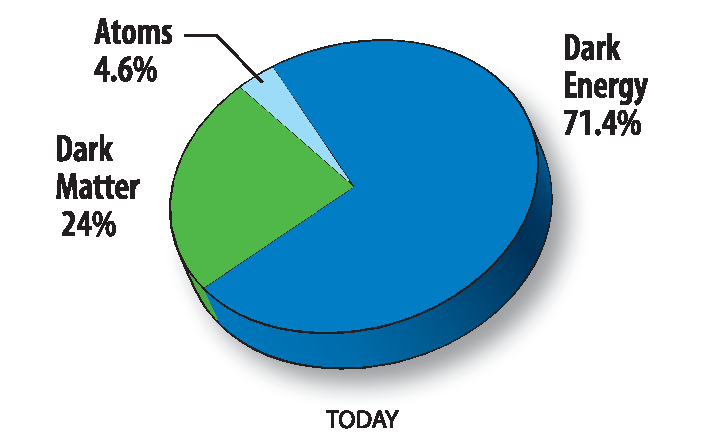
\includegraphics{figures/121236_NewPieChart.pdf}
%%This figure is from http://wmap.gsfc.nasa.gov/news/
%\caption{The universe is composed of normal matter ($\sim5\%$), dark matter ($\sim25\%$), and dark energy ($\sim70\%$). Figure adapted from \url{http://wmap.gsfc.nasa.gov/news/}.}
%\label{fig: the_composition_of_the_universe}
%\end{figure}
%Dark matter is a hypothetical particle which cannot be directly observed by telescopes because dark matter neither emits or absorbs light. Astrophysicists found the existence of dark matter from the large %discrepancies between the total mass calculated from star, gas, and dust and the mass of astronomical objects estimated from their gravitational effect.








% bibliography    
\begin{thebibliography}{999}
\bibitem{wess_and_zumino} Wess, J.; Zumino, B. (1974). "Supergauge transformations in four dimensions". Nuclear Physics B 70 (1): 39 $-$ 50.
%\bibitem{the_composition_of_the_universe} Figure adapted from http://wmap.gsfc.nasa.gov/news/
\bibitem{majorana} E. Majorana (1937), "Theory of the symmetry of electrons and positrons", Nuovo Cim. 14 (1937): 171 $-$184.
\bibitem{arXiv:1006.1718v2} Palash B. Pal (2010). "Dirac, Majorana and Weyl fermions". arXiv:1006.1718v2 [hep-ph] 12 Oct 2010.
\bibitem{Bilal} Adel Bilal. "Introduction to Supersymmetry". arXiv:hep-th/0101055v1 10 Jan 2001.
\bibitem{larsenf} \url{http://www-personal.umich.edu/~larsenf/Lecture1.pdf}
\bibitem{Martin} Stephen Martin. "A Supersymmetry Primer". arXiv:hep-ph/9709356v6 6 Sep 2011.
\bibitem{Pesink} Michael Peskin. "Supersymmetry in Elementary Particle Physics". arXiv:0801.1928 [hep-ph] 13 Jan 2008.
\bibitem{Drees} Manuel Dress. "An Introduction to Supersymmetry". arXiv:hep-ph/9611409v1 25 Nov 1996.
\bibitem{Dawson} S. Dawson. "Susy and such". arXiv:hep-ph/9612229v2 14 Jan 1997
\bibitem{Aitchison} Ian J. R. Aitchison. "Supersymmetry in Particle Physics An Elementary Introduction". SLAC-R-865 May 2007
\bibitem{Haber and Kane} Howard E. Haber; G.L. Kane. "The search for supersymmetry: probing physics beyond the standard model"
\bibitem{Pape and Treille} Lue Pape; Daniel Treille. "Supersymmetry facing experiment: much ado (already) about nothing (yet)". Rep. Prog. Phys. \textbf{69} (2006) 2843-3067
\bibitem{Jungman, Kamionkowski, Griest} Gerard Jungman, Marc Kamionkowski, Kim Griest. "Supersymmetric dark matter". Physics Reports 267 (1996) 195-373
\bibitem{O'Raifeartaigh} L. O'Raifeartaigh. '' Nucl. Phys. B \textbf{96}, 331 (1975)
\end{thebibliography}



\end{document}